\chapter{Experimentos Computacionais}
\label{cap:experimentos}
Com base na abordagem metodológica apresentada no Capítulo \ref{cap:abordagem_proposta}, os experimentos computacionais foram conduzidos da seguinte maneira. Inicialmente, apresenta-se o processo de construção do conjunto de dados, conforme detalhado na Seção \ref{sec:conjunto_dados_resultados}. Em seguida, na Seção \ref{sec:modelos_parametros_resultados}, são definidos os modelos empregados na tarefa de previsão, bem como os ajustes de hiperparâmetros realizados. A Seção \ref{sec:experimentos _metricas} discute como esses modelos serão avaliados e analisados. Por fim, os resultados experimentais são apresentados na Seção \ref{sec:resultados_experimentais}.


\section{Conjunto de Dados}
\label{sec:conjunto_dados_resultados}
Para a condução dos experimentos computacionais, foram selecionados três ativos financeiros: PETR3, WINFUT e WDOFUT. Amostras de cada ativo foram coletadas no período de 16/06/2021 até 16/06/2023 (2 anos) com granularidades de 30 e 60 minutos, totalizando 9156 amostras para granularidade de 30 minutos e 4664 para granularidade de 60 minutos.
Posteriormente, foram criadas novas variáveis com base nos valores de \ac{OHLC}, como descrito em detalhes na Seção \ref{subsec:feature_generate}. Essas variáveis foram então escolhidas para cada conjunto de modelos de previsão, conforme explicado na Seção \ref{sec:selecao_variaveis}, onde os parâmetros $x$ e $k$ foram definidos como 8 e 4, respectivamente.

Por fim, as seis bases de dados coletadas foram categorizadas cada uma em três segmentos distintos. Dessa forma, 10\% da base de dados foi reservada para a otimização dos modelos de previsão, 70\% destinou-se ao treinamento desses modelos, e os restantes 20\% compuseram ao segmento de teste. No caso das bases de dados com granularidade de 30 minutos, essa distribuição compreendeu 916 amostras para otimização, 6409 para treinamento e 1831 para teste. Para as bases de dados com granularidade de 60 minutos, a distribuição foi de 466 amostras para otimização, 3265 para treinamento e 932 para teste. Essas alocações podem ser visualizadas nas figuras \ref{fig:PETR3_fechamento}, \ref{fig:WINFUT_fechamento} e \ref{fig:WDOFUT_fechamento}, juntamente com a tendência de cada ativo e sua faixa de variação.

\subsection{PETR3}
No contexto do ativo financeiro PETR3, o processo de construção dos \textit{datasets} (\textit{dataset1} e \textit{dataset2}) resultou em conjuntos distintos de variáveis, influenciados pelas diferentes granularidades presentes nas bases de dados. Dessa maneira, as variáveis que compõem cada conjunto de dados são as seguintes:
\begin{itemize}
	\item \textbf{\textit{dataset1} (30 minutos):} \ac{ADX} com uma janela deslizante de 14, \ac{MACD} obtido a partir do valor de fechamento com janelas deslizantes de 8 e 17 amostras, além de duas variáveis relacionadas ao \ac{ROC}. Estas referem-se à derivada do valor máximo e do fechamento, ambas com janelas deslizantes de 10 amostras.
	
	\item \textbf{\textit{dataset2} (30 minutos):} \ac{K} com uma janela deslizante de 8 amostras, \ac{TSI} obtido a partir do valor de fechamento com janelas deslizantes de 13 e 25 amostras, e mais duas variáveis relacionadas ao \ac{R} com janelas deslizantes de 14 e 21 amostras.
	
	\item \textbf{\textit{dataset1} (60 minutos):} \ac{ADX} com uma janela deslizante de 14 amostras, \ac{ROC} com janela deslizante de 10 amostras, calculado a partir do valor de fechamento, e duas variáveis relacionadas ao \ac{MACD}, ambas derivadas do valor de fechamento. Uma delas com janelas deslizantes de 12 e 26 amostras, e a outra com uma janela deslizante de 8 e 17 amostras.
	
	\item \textbf{\textit{dataset2} (60 minutos):} \ac{ROC} derivado do valor de abertura com uma janela deslizante de 12 amostras, \ac{R} com uma janela deslizante de 5 amostras, e duas variáveis associadas a \ac{K}, uma com janelas deslizantes de 8 e 10 amostras.
\end{itemize}

\begin{figure}[htbp]
	\caption{Base de dados do ativo financeiro PETR3.}
	\centering
	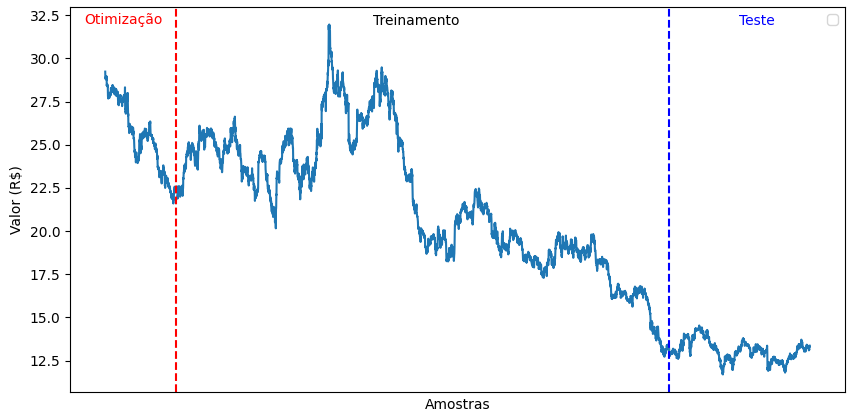
\includegraphics[width=.99\linewidth]{PETR3_fechamento.png} 
	\label{fig:PETR3_fechamento}
\end{figure}

\subsection{WINFUT}
Já no contexto do ativo financeiro WINFUT, o processo de construção dos \textit{datasets} (\textit{dataset1} e \textit{dataset2}) também resultou em conjuntos distintos de variáveis. Dessa maneira, as variáveis que compõem cada conjunto de dados são as seguintes:
\begin{itemize}
	\item \textbf{\textit{dataset1} (30 minutos):} \ac{ADX} com uma janela deslizante de 14 amostras, \ac{MACD} derivado do valor máximo com janelas deslizantes de 12 e 26 amostras, \ac{K} com uma janela deslizante de 8 amostras, e \ac{CCI} com uma janela deslizante de 18 amostras.
	
	\item \textbf{\textit{dataset2} (30 minutos):}  \ac{R} com uma janela deslizante de 5 amostras, \ac{TSI} derivado do valor de fechamento com janelas deslizantes de 13 e 25 amostras, \ac{K} com uma janela deslizante de 8 amostras, e \ac{SMA} com janela deslizante de 3 amostras.
	
	\item \textbf{\textit{dataset1} (60 minutos):} \ac{ADX} com uma janela deslizante de 14 amostras, \ac{CCI} com uma janela deslizante de 18 amostras, \ac{MACD} derivado do valor máximo com janelas deslizantes de 12 e 26 amostras, e \ac{K} com uma janela deslizante de 8 amostras.
	
	\item \textbf{\textit{dataset2} (60 minutos):} permanecem as variáveis do \textit{dataset1} de 30 minutos, com exceção da variável \ac{K}, que neste \textit{dataset} possui uma janela deslizante de 14 amostras.
\end{itemize}

\begin{figure}[htbp]
	\caption{Base de dados do ativo financeiro WINFUT.}
	\centering
	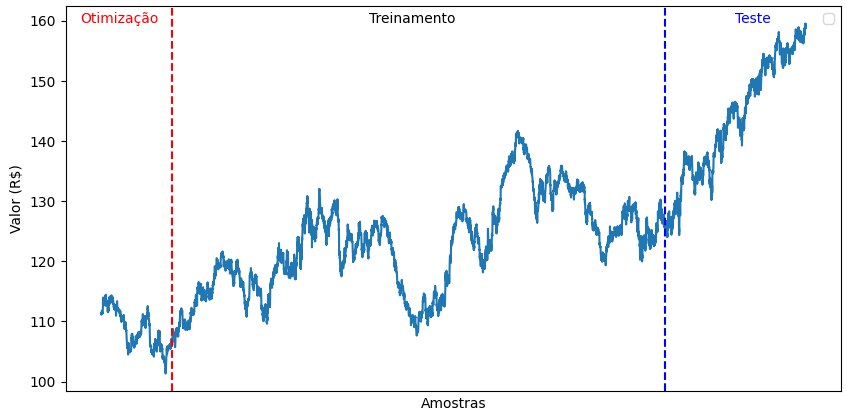
\includegraphics[width=.99\linewidth]{WINFUT_fechamento.png} 
	\label{fig:WINFUT_fechamento}
\end{figure}

\subsection{WDOFUT}
Por fim,  para o ativo financeiro WDOFUT, o processo de construção dos \textit{datasets} (\textit{dataset1} e \textit{dataset2}) também conduziu à formação de conjuntos únicos de variáveis. Desse modo, as variáveis que integram cada conjunto de dados são as seguintes:
\begin{itemize}
	\item \textbf{\textit{dataset1} (30 minutos):} \ac{ADX} com uma janela deslizante de 14 amostras, \ac{MACD} calculado a partir do valor máximo com janelas deslizantes de 12 e 26 amostras, \ac{K} com uma janela deslizante de 8 amostras, e \ac{CCI} com uma janela deslizante de 18 amostras.
	
	\item \textbf{\textit{dataset2} (30 minutos):} \ac{ADX} com uma janela deslizante de 14 amostras, \ac{ROC} obtida a partir do valor máximo com uma janela móvel de 10 amostras, e duas variáveis de \ac{MACD}. Ambas são derivadas do valor máximo, sendo uma com janelas deslizantes de 8 e 17 amostras, e a outra com janelas deslizantes de 12 e 26 amostras.
	
	\item \textbf{\textit{dataset1} (60 minutos):} \ac{ADX} com uma janela deslizante de 14 amostras, \ac{CCI} com uma janela deslizante de 18 amostras, \ac{MACD} obtido a partir do valor máximo com janelas deslizantes de 12 e 26 amostras, e \ac{K} com uma janela deslizante de 8 amostras.
	
	\item \textbf{\textit{dataset2} (60 minutos):} \ac{ADX} com uma janela deslizante de 14 amostras, \ac{ROC} calculada a partir do valor máximo com uma janela deslizante de 12 amostras, \ac{K} com uma janela deslizante de 10 amostras, e \ac{MACD} derivado do valor máximo com janelas deslizantes de 12 e 26 amostras.
\end{itemize}

\begin{figure}[htbp]
	\caption{Base de dados do ativo financeiro WDOFUT.}
	\centering
	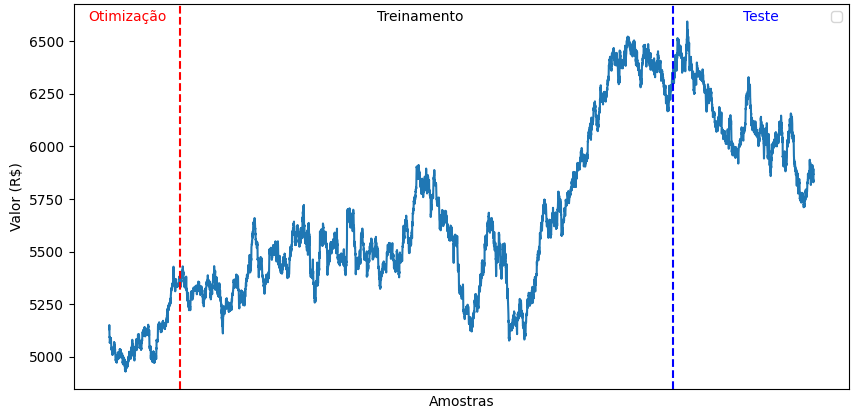
\includegraphics[width=.99\linewidth]{WDOFUT_fechamento.png} 
	\label{fig:WDOFUT_fechamento}
\end{figure}


\section{Modelos e Hiperparâmetros}
\label{sec:modelos_parametros_resultados}
Para efetivar a proposta delineada na Seção \ref{sec:previsao}, foram empregados 10 modelos distintos de previsão. No grupo de modelos estatísticos, destacam-se três escolhas específicas: \ac{ARIMA}, \ac{SARIMA}, e \ac{GARCH}. O conjunto de modelos de classificação compreende outros três: \ac{SVM}, \ac{KNN}, e \ac{LR}, enquanto o conjunto de modelos de regressão é representado por \ac{LSTM}, \ac{MLP}, e \ac{RNN}. Além disso, concebeu-se um modelo final, uma \ac{MLP} denominada "MLP out", cuja função é consolidar os resultados provenientes de cada ensemble dos três conjuntos mencionados anteriormente.
A Tabela \ref{tab:hyperparam_otmz} detalha a estrutura de cada modelo de previsão, juntamente com o processo de otimização implementado e as escolhas otimizadas para cada conjunto de dados coletado. 

\LTXtable{\textwidth}{content/tabela_hyperparam}
	
\section{Experimentos e Métricas}
\label{sec:experimentos _metricas}
As métricas de avaliação desempenham um papel crucial na análise meticulosa dos modelos propostos, sendo aplicadas em três categorias distintas: modelos de classificação, modelos de regressão e estratégia de compra e venda.
Na avaliação dos modelos de regressão:  \ac{GARCH}, \ac{ARIMA}, \ac{SARIMA}, \ac{LSTM}, \ac{MLP}, \ac{RNN} e \ac{MLP} Out . A escolha recaiu sobre as métricas de \ac{MAE} e \ac{RMSE}. Essas métricas foram selecionadas devido à sua capacidade de proporcionar uma representação direta dos erros, conferindo maior relevância aos erros mais impactantes. Essa abordagem busca proporcionar uma compreensão clara e detalhada do desempenho de cada modelo, permitindo uma análise aprofundada das discrepâncias entre as previsões e os valores reais.

Já na fase de avaliação dos modelos de classificação, todos os modelos definidos serão considerados, uma vez que a função de transformação que converte resultados de regressão em classificação é aplicada uniformemente a todos os modelos de regressão. Para a avaliação desses modelos, serão utilizadas métricas como Acurácia, \ac{F1} e Matriz de Confusão. A Acurácia proporciona uma visão global da precisão do modelo, enquanto a métrica \ac{F1} equilibra precisão e recall. A Matriz de Confusão oferece uma análise mais detalhada do desempenho do modelo em diferentes categorias, possibilitando uma compreensão mais completa de seu comportamento em situações de classificação. 

Por fim, todos os modelos e ensembles definidos durante o experimento serão avaliados com base na estratégia delineada na Seção \ref{sec:estrategia}, permitindo a comparação do percentual de retorno de cada modelo ao final da execução, juntamente com a quantidade de operações de compra realizadas. Essa análise final busca fornecer \textit{insights} valiosos sobre a eficácia prática de cada abordagem na execução da estratégia proposta.

\section{Resultados Experimentais}
\label{sec:resultados_experimentais}
\subsection{PTR3}´
\subsubsection{Regressão}
\subsubsection{Classificação}
\subsubsection{Recomendação de Investimento}
\subsection{WINFUT}
\subsubsection{Regressão}
\subsubsection{Classificação}
\subsubsection{Recomendação de Investimento}
\subsection{WDOFUT}
\subsubsection{Regressão}
\subsubsection{Classificação}
\subsubsection{Recomendação de Investimento}


